\chapter{Data Acquisition}\label{c:daq}

\section{Data Acquisition Systems}
Figure~\ref{f:daq} illustrates a typical \gls{data acquisition system} which consists of the following components:
\begin{itemize}
\item Sensor(s): Device for converting a physical quantity into an analog signal, e.g., accelerometer, thermocouple or strain gage.
\item Signal Conditioning: Electronics for adapting sensor output to comply with the input of a DAC, e.g., filtering, Wheatstone bridge or amplification.
\item Digital-to-Analog Converter (DAC): See Section~\ref{s:dac}.
\item Destinations: Digital display (e.g., 2D graph) or archive (e.g., log file).
\end{itemize}

\begin{figure}[hbt!]
\centering
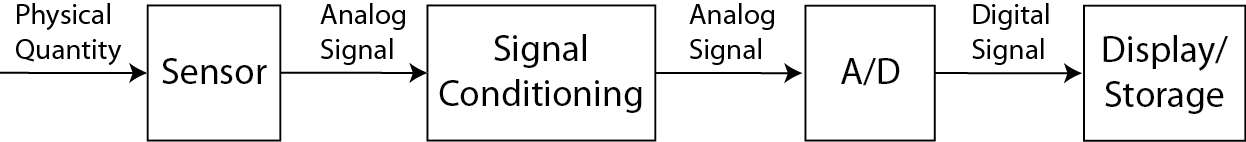
\includegraphics[width=\FigWidth\textwidth]{daq.png}
\caption{Simple data acquisition system diagram.}
\label{f:daq}
\end{figure}

In this chapter we'll work through each of the subsystems in Figure~\ref{f:daq} to discuss how they operate together to create a system for making digital measurements.

\section{Sensors}
A \gls{transducer} is a device that converts one type of energy into another type of energy.  A sensor is a transducer, but not all transducers are sensors.  (The opposite of a sensor is an actuator).  Here are some examples:
\begin{itemize}
\item A microphone is a transducer that converts acoustic energy (sound pressure) to electrical energy (voltage). A microphone is a sensor.
\item A speaker is a transducer that converts electrical energy to acoustic energy.  A speaker is an actuator.
\item An accelerometer is a transducer that converts mechanical energy (vibration) to electrical energy (voltage).  An accelerometer is a sensor.
\item An electric motor is a transducer that converts electrical energy to mechanical energy (rotation).  An electric motor is an actuator.
\item A thermocouple is a transducer that converts thermal energy (temperature) to electrical energy (voltage).  A thermocouple is a sensor.
\item A heating coil is a transducer that converts electrical energy to thermal energy.  A heating coil is an actuator.
\end{itemize}

\begin{ex}
Following the pattern in the list above, list two more transducers that are sensors and two more transducers that are actuators.
\end{ex}


There are many, many types of sensors.  For just about everything we can imagine wanting to measure there is a device that will convert the physical parameter to an electrical signal that we can use for data aquisition.  For our purposes we will focus on sensors that measure mechanical quantities (motion, strain, temperature, etc.) by producing an electrical output.  The next step is converting that electrical output into a form that our D/A can accept.  

\subsection{Sensitivity}
The sensitivity of a sensor is the parameter of the sensor that describes the transduction.  In simple cases the sensitivity of a sensor is given as a ratio between the output (typically voltage) and the physical input.  For example, the ADXL 335 accelerometer has a typical sensitivity of \unitfrac[300]{mV}{g} which means that for an input acceleration of \unit[1.0]{g} the sensor output will be \unit[300]{mV}.
\begin{ex}\label{ex:asens}
Suppose we are going to use an ADXL 335 accelerometer to measure the acceleration of a radio-controlled car.  We know that the car has a maximum forward acceleration of \unitfrac[2.5]{m}{s$^2$}.  What is the maximum output voltage we could expect from the accelerometer?
\end{ex}
\begin{ex}
A Type K thermocouple is a common sensor for measuring temperature, and the typical sensitivity for such a device is \unitfrac[41]{$\mu$V}{$^{\circ}$C}.  What output voltage could we expect if we were using this device to measure the temperature of boiling water (at sea-level)?
\end{ex}

A complication that can arise is when the sensitivity of a sensor is not a constant.  This can happen if there is a non-linear relationship between the physical parameter and the output.  In this case we may have to use a mathematical relation (i.e., a formula, hopefully supplied by the sensor datasheet) to convert the output signal (voltage) to the physical measurement.  Another situation is when the output depends on the supplied voltage, which is called a \gls{ratiometric} sensitivity.  In fact, I oversimplified the ADXL 335 sensitivity.  This sensor requires a supply voltage, sometimes referred to as the \gls{excitation voltage}, to power the sensor.  The typical supply voltage is \unit[3.0]{V}, but the value can range between \unit[1.8--3.6]{V}.  The sensitivity is directly proportional to this supply voltage, so with a supply of \unit[1.8]{V} we can expect a sensitivity of \unitfrac[180]{mV}{g}.  

Another common example of a ratiometric sensitivity is a load cell.  As its name implies, a load cell is a sensor that reports a load (tension or compression) as a voltage.  A common type of load cell is S-Beam load cell that uses a configuration of strain gages to measure the strain in a mechanical beam.  The beam is calibrated so that the relationship between the strain and the applied force is known.  The sensitivity of this type of sensor is specified in a confusing manner.  For example, a typical device will come in a range of load capacities, say \unit[25-10,000]{lb}.  For this family of devices the sensitivity might be quoted as \unitfrac[3]{mV}{V}.  What on earth does this mean you ask?  Well, it means that at the maximum load, the output voltage is \unit[3]{mV} multiplied by the excitation voltage.  They typical excitation voltage of this particular device is \unit[10]{V}.  So, if we have a load cell rated at \unit[100]{lb} and we apply the recommended excitation of \unit[10]{V}, the sensitivity is \unitfrac[0.3]{mV}{lb}.  In other words, we can find the sensitivity (\unitfrac[S]{mV}{lb}) as
\begin{equation}\label{e:sens}
\unitfrac[S]{[mV}{lb]} = \frac{(\unitfrac[O]{[mV}{V]})(\unit[E]{[V]})}{\unit[L_{max}]{[lb]}}
\end{equation}
where \unitfrac[O]{[mV}{V]} is the ratiometric output of the load cell, \unit[E]{[V]} is the excitation voltage and \unit[L$_{\mathrm{max}}$]{[lb]} is the maximum load capacity for the device.
\begin{ex}
Suppose we want to use two AA alkaline batteries to power our ADXL 335 accelerometer.  What sensitivity could we expect with this arrangement?
\end{ex}
\begin{ex}
Consider that we are using a thin-beam load cell (Omega LCL Series) with a maximum load capacity of \unit[1]{lb}.  The rated output of the load cell is \unitfrac[2]{mV}{V} and the recommended excitation is \unit[5]{V}.  
\begin{itemize}
\item What is the sensitivity of the load cell in \unitfrac[]{mV}{lb}?
\item What is the maximum voltage we could expect when the load cell is at its maximum capacity load?
\item What is the voltage we could expect if we apply a \unit[0.25]{lb} load?
\end{itemize}
\end{ex}

\ifsolutions
\begin{soln}
The sensitivity is calculated using (\ref{e:sens}).
\[
\unitfrac[S]{[mV}{lb]} = \frac{(\unitfrac[2.0]{[mV}{V]})(\unit[5.0]{[V]})}{\unit[1.0]{[lb]}} = \unitfrac[10.0]{mV}{lb}
\]

The maximum voltage is the product of the maximum load and the sensitivity.
\[
V_{max} = \unitfrac[10]{mV}{lb} (\unit[1]{lb}) = \unit[10]{mV}
\]

Again, this is the product of the senitivity and the load.
\[
V_{max} = \unitfrac[10]{mV}{lb} (\unit[0.25]{lb}) = \unit[2.5]{mV}
\]
\end{soln}
\fi


\section{Signal Conditioning}
Sensors often have an output that is inconvenient to use with digital-to-analog converters.  As we alluded to in Chapter~\ref{c:measure}, digital-to-analog converters typically take a voltage as input and it is important that we use the full range of the voltage that the D/A will accept (e.g., \unit[0--10]{V}).  

Consider the case of a strain gage, illustrated in Figure~\ref{f:condition}.  The specifics will be discussed in more detail later, but for now it will suffice to say that a strain gage is a sensor that converts a strain (a change in length) to a change in electrical resistance.  This is great, but how do we plug that into our D/A which wants a voltage between \unit[0--10]{V}?  It turns out that Sir Charles Wheatstone found a solution to this problem in an elegant circuit that is now called the Wheatstone bridge.  This circuit converts the change in resistance to a very small voltage, say \unit[0--10]{mV}.  Now we have another problem, our D/A wants a much larger voltage that the \unit[10]{mV} coming from the Wheatstone bridge.  Perhaps we could add an amplifier that will multiply the output of the bridge by a gain of 1,000 so that we now have a  voltage that is suitable for the D/A.  

\begin{figure}[hbt!]
\centering
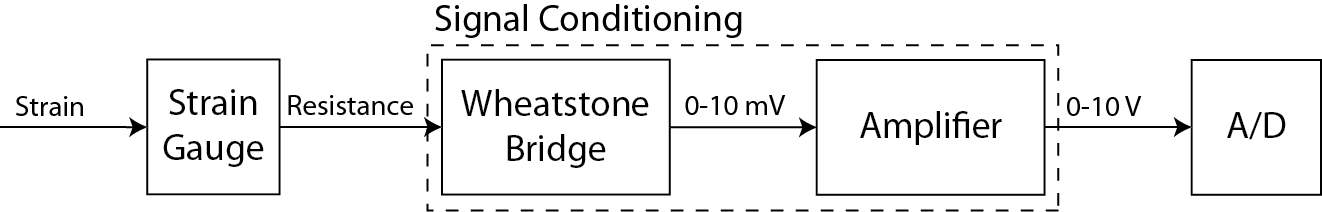
\includegraphics[width=\FigWidth\textwidth]{condition.png}
\caption{Signal conditioning example.  In the case of the strain gage, a Wheatstone bridge and amplifier are used to condition the signal before it is passed to the analog-to-digital converter.}
\label{f:condition}
\end{figure}

For our purposes two general types of signal conditioning will play an important role in designing our measurement systems, amplification and anti-aliasing.  For now we'll discuss amplification and we'll save the topic of anti-aliasing for Section~\ref{s:alias}.

\subsection{Amplifiers}
The role of an amplifier in our signal conditioning system is to scale the electrical output of a sensor (typically voltage) to match the input range of the analog-to-digital converter.  As we discussed in Section~\ref{s:dac}, in order to take full advantage of the resolution of our A/D, the signal range must be approximately equivalent to the input range of our A/D.  In theory (always a dangerous first two words), the function of an amplifier is to provide a multiplicative gain in the signal path, i.e., 
\[
V_{out} = K\left(V_{in}\right)
\]
where $V_{in}$ is the input to the amplifier, $V_{out}$ is the amplifier output and $K$ is the amplifier gain. 

\begin{ex}
Building on Exercise~\ref{ex:asens} consider that we want to interface our ADXL 335 into an A/D that has a range of \unit[0--10]{V} and 12-bits of resolution.  
\begin{itemize}
\item If we did not use any amplification, what would be the effective resolution (in bits) of our A/D?  (Hint: See Section~\ref{s:dac}.)
\item What amplifier gain would you suggest so that we could use the full resolution of the A/D?
\end{itemize}
\end{ex}

\section{Analog-to-Digital Conversion}
We started our discussion of A/D devices in Section~\ref{s:dac}.  Here we'll add some detail to our description of these devices.  Again, we'll focus on \emph{what} these devices do and leave the specifics of \emph{how} they do this (successive-approximation, sigma-delta, etc.) to another book.
\subsection{Range and Resolution}
Recall that the function of an ADC is to convert an voltage input (analog) to a binary number (digital).  The \gls{full scale voltage range} ($E_{\mathrm{FSR}}$) is the span of voltage inputs that the A/D will accept.  This range comes in two flavors: bilateral or unilateral.  A bilateral input range is typically symmetric about \unit[0]{V} while a unilateral input can only accept positive voltage values.  For example,
\begin{itemize}
\item Bilateral Input Range: $\pm$\unit[10]{V}
\item Unilateral Input Range: \unit[0--10]{V}
\end{itemize}
In either case the full scale range is simply $E_{\mathrm{FSR}}=V_{\mathrm{max}}-V_{\mathrm{min}}$ where the maximum input voltage is $V_{\mathrm{max}}$ and the minimum input voltage is $V_{\mathrm{min}}$.  
\begin{ex}
For the bilateral and unilateral examples above what is $E_{\mathrm{FSR}}$ for each case?
\end{ex}

Any voltage within the input range is converted to a binary value.  The length of this binary number is specified by the number of bits ($M$) inherent to the A/D, e.g., 12-bits.  The length of the binary representation determines the finite number of voltage levels that can be represented (see Section~\ref{s:dac}), so the ratio of the full scale voltage range to the number of levels that we can use in that range determines the resolution $Q$ (in Volts) of the A/D,
\begin{equation}
\label{e:q}
Q = \frac{E_{\mathrm{FSR}}}{2^M}.
\end{equation}
You might notice that the resolution of an A/D is often referred to as either the number of bits used in the conversion ($M$) or the resolution in volts ($Q$).  This is somewhat sloppy nomenclature, but common. 

A related concept is \myglssym{quantization error} which is another way of describing the finite resolution of converting a continuous analog value to a discrete digital value.  As we discussed in Section~\ref{s:dac}, the A/D will associate the incoming voltage level (which can assume an infinite number of possible values) with the binary representation (which can only assume one of $2^M$ possible values) that is nearest that actual value.  Based on this nearest-neighbor concept the error between the actual incoming analog voltage and the reported digital value will be $\pm Q/2$, the quantization error.


\begin{ex}
An alternative to (\ref{e:q}) is to express the resolution as 
\[
Q = \frac{E_{\mathrm{FSR}}}{2^M-1}.
\]
\begin{itemize}
\item Can you explain why this might be more correct?  Try drawing a picture of a 1-bit or 2-bit scenario to understand why we might actually only have $2^M-1$ levels in our A/D.
\item Given that typical A/D hardware has more than 10-bits, and as much as 24-bits, of resolution, is the difference between these alternatives significant?  Why or why not?
\end{itemize}
\end{ex}

\ifsolutions
\begin{soln}

There are many answers to this.  The point is that the student think about what is going on here.
\begin{itemize}
\item In general, for an $M$-bit A/D there are $2^M$ possible outputs.  However, the distance between each level is $E_{FSR}/(2^M-1)$ which is more correctly associated with the resolution of the A/D
\item For any reasonably large number of bits there the is a negligible difference between these expressions.  For example, $2^{24}=16,777,216$ and $2^{24}-1=16,777,215$.  The point is that either expression is sufficient.
\end{itemize}
\end{soln}
\fi

\subsection{Differential Versus Single-Ended}
When connecting a voltage input to an A/D there are two important options: differential or single-ended input. \Gls{single-ended input} consists of a common ground (GND) that is shared between all the inputs to the A/D.  The A/D output is based on the voltage measured between the signal input (+) and ground.  In contrast \gls{differential input} consists of two voltage inputs, high (+) and low (-), which may or may not be referenced to a common GND potential.  The A/D output is then based on the voltage difference (hence differential) between the signal high and signal low potentials.  Here are some advantages of each approach:
\begin{itemize}
\item Single-ended inputs are simpler to implement
\item Single-ended inputs use the full number of channels in the A/D device. For example, a device advertised to have ``16 inputs'' will actually have 16 single-ended inputs, but only 8 differential inputs.
\item Single-ended inputs are lower in cost
\item Differential inputs are less susceptible to noise (electromagnetic or radio-frequency interference).  This is particularly important for sensors that produce very small signals, e.g., strain gages, thermocouples, load cells, etc.
\item Differential inputs can be applied in cases (such as Wheatstone bridge outputs) where there is no true connection to a common ground.
\end{itemize}

\subsection{Sampling}
So far we have been concerned with the resolution of a digital measurement in terms of the finite levels, typically of voltage, that an ADC can use to represent the analog input---the y-axis in Figure~\ref{f:sample}.  In this section we'll discuss the ramifications of the fact that the ADC operates at a finite \gls{sampling period} ($dt$), the output of the ADC changes only at discrete times.  Therefore, an ADC has finite resolution in both amplitude (i.e., voltage) and time, illustrated by the fact that the individual samples in Figure~\ref{f:sample} are discrete points in the x and y axes.
\begin{figure}[hbt!]
\centering
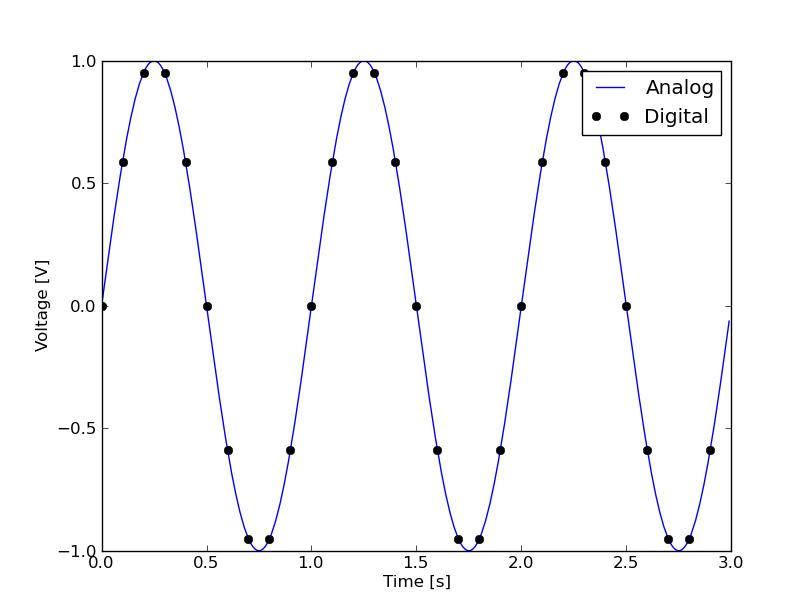
\includegraphics[width=\FigWidth\textwidth]{sample.png}
\caption{Illustration of a sampled signal.  The analog signal ($y(t)=\sin{\omega t}$) is represented by a continuous curve with an infinite set of values in both time (x-axis) and amplitude (y-axis).  The A/D converts this signal discrete samples at a finite set of time and amplitude values.}
\label{f:sample}
\end{figure}

The typical function of an A/D is to regularly sample the input voltage level and record these samples as digital numbers.  The speed at which this happens is specified by the sampling rate, or equivalently the \gls{sampling frequency} ($f_s$) where \unit[$f_s=dt$]{Hz}. (Beware, the terms ``sample rate'' or ``sampling rate'' are often used to refer to both sampling period and sampling frequency.)  The sampling is illustrated in Figure~\ref{f:sample} by the black markers; the time between each sample ($dt=\unit[0.1]{s}$) is the sampling period.


\begin{figure}[hbt!]
\centering
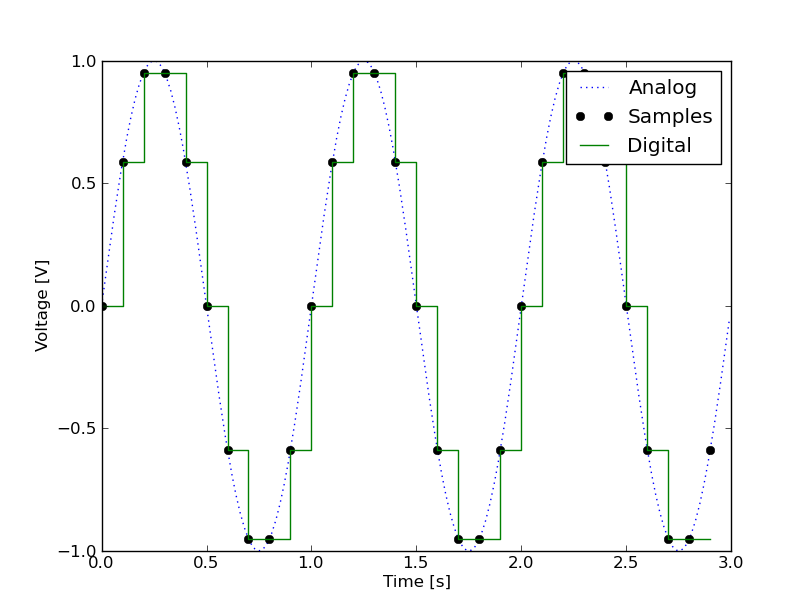
\includegraphics[width=\FigWidth\textwidth]{sample2.png}
\caption{A second illustration of the sampled signal from Figure~\ref{f:sample}. The ``Digital'' graph shows how the digital output of the A/D changes over time.  The reported value from the A/D only changes after each sampling event.}
\label{f:sample2}
\end{figure}

\begin{ex}
Consider the same analog input as illustrated in Figure~\ref{f:sample} and Figure~\ref{f:sample2}, a continuous sine wave input with a period of \unit[1.0]{s} and an amplitude of \unit[1.0]{V}.  The signal is input to a A/D with the following characteristics:
\begin{itemize} 
\item 4-bit voltage resolution
\item $E_{\mathrm{FSR}}= \pm \unit[1.0]{V}$
\item $dt = \unit[0.5]{s}$
\end{itemize}
Sketch a 2D graph (Voltage versus Time) that illustrates the analog signal and the digital samples.

\vspace{1ex}

Sketch the same 2D graph if $dt=\unit[0.33]{s}$.
\end{ex}

\subsection{How Fast to Sample?}
The sampling rate (see the warning above!) for A/D devices can vary by orders of magnitudes. Consider the contrast between two processes that we might want to measure: the rise of global temperature or the incoming voice signal from an iPhone user.  These processes evolve on very different time-scales.  To measure global temperature rise it might be sufficient to take an average measurement once per year, but a typical sampling frequency for audio input is 44,000 samples-per-second (Hz).  

\begin{ex}
Suppose we wanted to sample the global temperature at a sampling frequency of \unit{44}{kHz} using a 16-bit A/D for a year.  Estimate the size of the hard drive (in bytes) that would be necessary to store this much data.  (Hint: There are 8-bits per byte.)
\end{ex}

The sampling frequency (or period) can often be specified in software when using a ADC.  So what setting should we choose?  The simple answer is that we typically sample as fast as we can!

The longer (and hopefully more interesting) answer is that we can set a minimum necessary sampling frequency based on the characteristics of the input signal.  Let's start with our audio (iPhone) example.  The key thing you need to know is that the typical range of human hearing is from \unit[20--20,000]{Hz}.  So we'll need to sample fast enough that our digital representation (the output of the ADC) can represent this complete frequency range.  It turns out that if we collect samples at \emph{twice} the maximum frequency of interest, then we will be able to represent the analog signal with our digital representation, i.e.,
\[
f_s \geq 2\left(f_{\mathrm{max}}\right)
\]
where $f_{\mathrm{max}}$ is the \gls{Nyquist frequency}, the maximum frequency of interest in the analog signal we are trying to measure.  The Nyquist frequency dictates the theoretical minimum required sampling frequency, but in practice we can often sample much faster than this minimum; a typical rule-of-thumb is to set $f_s = 10(f_{\mathrm{max}})$

\begin{ex}
What would be the minimum sampling frequency for the analog signal illustrated in Figure~\ref{f:sample}?  What would be the cooresponding Nyquist frequency?
\end{ex}

\ifsolutions
\begin{soln}
The signal in the figure has a single frequency of \unit[1]{Hz}; this is the Nyquist frequency.  To create a digital representation of this signal we'd need to sample at a minimum rate of \unit[2]{Hz}.
\end{soln}
\fi

\subsection{Anti-Aliasing}\label{s:alias}
What happens when we violate this sampling rule-of-thumb?  Let's work through an illustrative example similar to the illustration from Figure~\ref{f:sample}. Considering our simple sine wave input that changes amplitude with a frequency of \unit[1.0]{Hz}.  If we use our rule-of-thumb and set the sampling frequency to $f_s=\unit[10]{Hz}$ we will end up with a digital representation, illustrated in Figure~\ref{f:alias_x10}, that looks pretty much like the original analog signal.  \emph{If we sample ``fast enough'' the digital output will be a close approximation to the analog input.} 
\begin{figure}[hbt!]
\centering
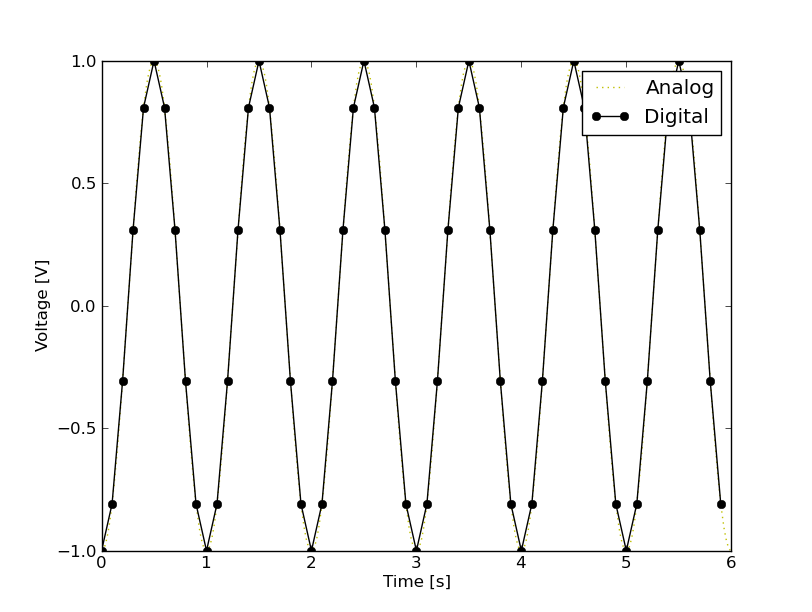
\includegraphics[width=\FigWidth\textwidth]{alias_x10.png}
\caption{A second illustration of the sampled signal from Figure~\ref{f:sample}. The ``Digital'' graph shows how the digital output of the A/D changes over time.  The reported value from the A/D only changes after each sampling event.}
\label{f:alias_x10}
\end{figure}

Now let's see how things change if we cut it close and use the minimum frequency ($f_s=\unit[2]{Hz}$), i.e., set the sampling frequency equal to twice the Nyquist frequency. Figure~\ref{f:alias_x1} illustrates that the sampled signal still roughly resembles the original sine wave, but things are starting to look a bit fishy.   
\begin{figure}[hbt!]
\centering
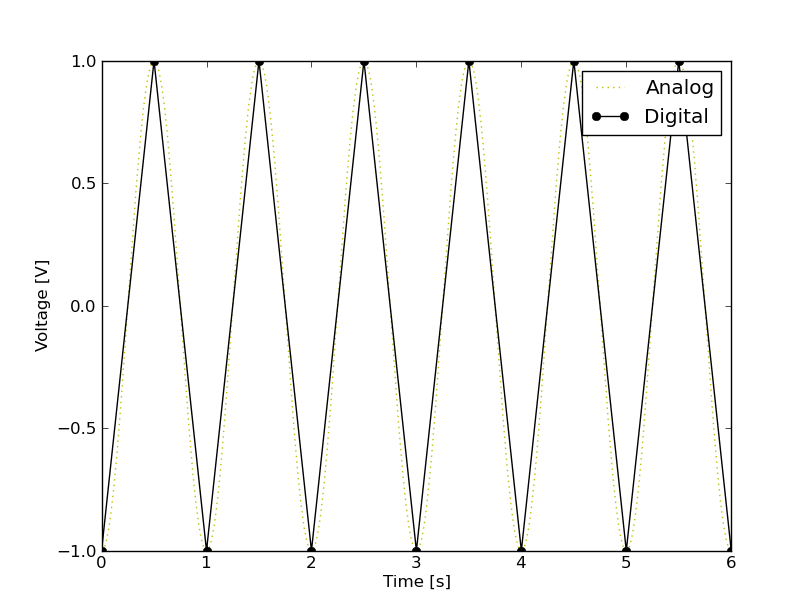
\includegraphics[width=\FigWidth\textwidth]{alias_x1.png}
\caption{Sampling at the minimum frequency, twice the Nyquist frequency: $f_s=\unit[2]{Hz}$, $dt=\unit[0.5]{s}$.}
\label{f:alias_x1}
\end{figure}

Finally, the sampling frequency becomes less than twice the Nyquist frequency the digital output is significantly different than the analog input.  Figure~\ref{f:alias_alias} illustrates that the digital output appears to be a sawtooth pattern with a much slower frequency of oscillation than the analog input, the term for this phenomenon is \gls{aliasing}.
\begin{figure}[hbt!]
\centering
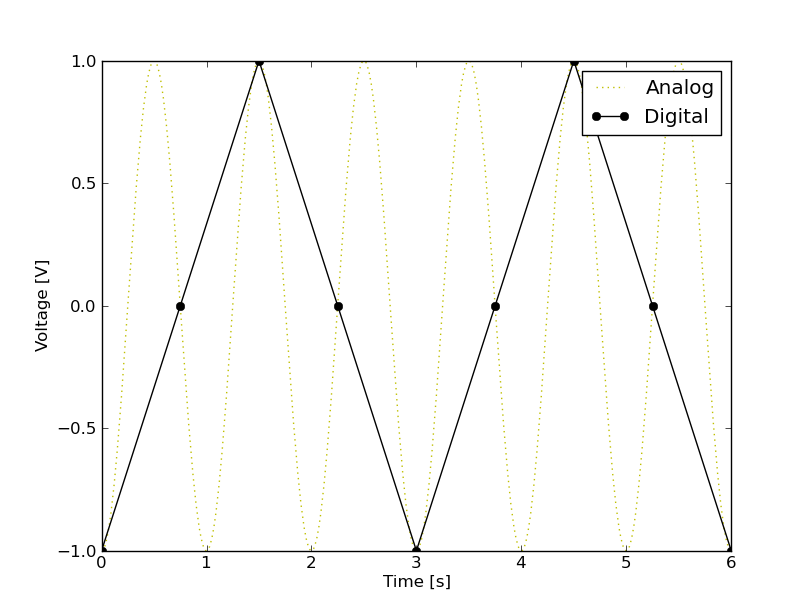
\includegraphics[width=\FigWidth\textwidth]{alias_alias.png}
\caption{Sampling below twice the Nyquist frequency: $f_s=\unit[1.33]{Hz}$, $dt=\unit[0.75]{s}$.}
\label{f:alias_alias}
\end{figure}

To generalize from our specific example, aliasing is when the analog input has significant frequency content above the half the sampling frequency.  These portions of the signal are folded back into the digital representation as lower frequency components that can corrupt the digital representation.  This can be a particular problem when there is high frequency noise.  In this case aliasing can cause high frequency noise to corrupt your lower frequency data.

To address this issue an anti-aliasing filter is often included in the signal conditioning portion of the data acquisition system.  This analog low-pass filter attenuates the higher frequency portions of the analog input, those portions of the input above the Nyquist frequency, to prevent these high frequency portions of the input from corrupting the measurement.

\begin{ex}
Anti-aliasing filters must be implemented on the analog signal.  However, digital filters can be used on the digital measurement (after the A/D conversion).  Why is it not possible to have a digital anti-aliasing filter?
\end{ex}



